\documentclass[10pt, aspectratio=169]{beamer}

% Configuration {{{
\usepackage[utf8]{inputenc}
\usepackage[T2A]{fontenc} % T1 for English
\usepackage[english, russian]{babel}

\usepackage{mathtools}
\usepackage{graphicx}
\usepackage{tikz}
\usepackage[multidot]{grffile}
\usepackage[labelsep=period]{caption}
\usepackage{multirow}

\setbeamertemplate{caption}[numbered]
\setbeamertemplate{navigation symbols}{}
\usefonttheme[onlymath]{serif}
\usepackage{DejaVuSansCondensed} % helvet for English
\usetheme{Madrid}

\linespread{1.2}
% }}}

% Title and other {{{
\title[Measurements of BRs and studies of $\Lambda_c^+\pi^-$ resonances]{
  Measurements of
  $\mathcal{B}\big(\overline{B}{}^0 \rightarrow \Lambda_c^+\bar{p}\big)$
  and
  $\mathcal{B}\big({B}^- \rightarrow \Lambda_c^+\bar{p}\pi^-\big)$
  and studies of $\Lambda_c^+\pi^-$ resonances
  by BaBar Collaboration
  -- contents analysis
}
\author[Kerim Guseynov]{
  Kerim Guseynov \\[2ex] Based on \texttt{arXiv:0807.4974}
}
\institute[MSU]{
  Faculty of Physics \\ Moscow State University
}
\date{Nov 18, 2022}
%}}}

\begin{document}

\frame[plain]{\titlepage}

\begin{frame}[label=intro]%{{{
  \frametitle{Introduction}

  \large
  \begin{itemize}
    \item Complementary measurements to heavy baryon decays,
      \vskip 2ex
    \item Baryon production mechanisms:
      \\ suppression of decays like $B \to p\bar{p}$ vs $B \to 
      p\bar{p}\pi$,
      \vskip 2ex
    \item Scalar mesons simplify spin measurements,
  \end{itemize}

  % Perhaps the most satisfying theoretical interpretation of baryonic 
  % B decay rates is the qualitative one proposed by Hou and Soni in 
  % 2001 [16], who argue that B decays are favored if the baryon and 
  % antibaryon in the final-state configuration are close together in 
  % phase space. A consequence is that decay rates to two-body 
  % baryon-antibaryon final states are suppressed relative to rates of 
  % three-body final states containing the same baryon-antibaryon system 
  % plus an additional meson. In the three-body case, the baryon and 
  % antibaryon can be in the favored configuration—close to- gether in 
  % phase space—rather than back-to-back as in the two-body case
\end{frame}%}}}

\begin{frame}[label=babar]%{{{
  \frametitle{{BaBar} detector and data sample}
  \centering
  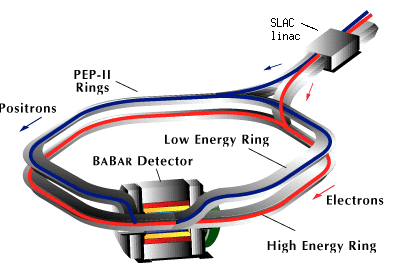
\includegraphics[width=.4\textwidth]{figures/002/babar-scheme}
  \hfill
  
\includegraphics[width=.56\textwidth]{figures/002/upsilon}

  \vskip 2ex
  $383$ million $\Upsilon(4S) \to B\overline{B}$ decays

  \vskip 3ex \hfill\null
  \textbullet{} Vertex tracker \hfill\hfill
  \textbullet{} Drift chamber \hfill\hfill
  \textbullet{} Cherenkov detector \hfill\null

  % The measurements presented in this paper are based on 383 × 10 
  % 6 Υ (4S) → BB decays recorded with the B A B AR detector [18] at the 
  % PEP-II e+ e− asymmetric-energy B Factory at the Stanford Linear 
  % Accelerator Center. At the interaction point, 9- GeV electrons 
  % collide with 3.1- GeV positrons at the Υ (4S) resonance with 
  % a center-of- mass energy of 10.58 GeV/c2 .
  % Charged particle trajectories are measured by a five- layer silicon 
  % vertex tracker (SVT) and a 40-layer drift chamber (DCH) immersed in 
  % a 1.5-T axial magnetic field. Charged particle identification is 
  % provided by ionization energy (dE/dx) measurements in the SVT and 
  % DCH along with Cherenkov radiation detection by an internally 
  % reflecting ring-imaging detector (DRC).
  %
  % Exclusive B-meson decays are simulated with the Monte Carlo (MC) 
  % event generator EvtGen [19]. Back- ground continuum MC samples (e+ 
  % e− → qq, where q = u, d, s, c) are simulated using Jetset7.4 [20] to 
  % model generic hadronization processes. Background MC samples of e+ 
  % e− → B + B − and B 0 B0 are based on simu- lations of many exclusive 
  % B decays (also using EvtGen). The large samples of simulated events 
  % are generated and propagated through a detailed detector simulation 
  % using the GEANT4 simulation package [21].
  %
  %
  %
  %  + +0we reconstruct + Λc candidates in the pK −π , pKS 0, pK S π+ π− 
  %  , and Λπ decay modes, requiring the in- variant mass of each Λ+ 
  %  c candidate to be within 10 MeV/c 2 of the world average value [8].
  %
  %  For B − + → − Λc + + pπ − , we also reconstruct Λ+ c candidates in the 
  %  Λπ π π decay mode, and require all of the Λc + candidates to have an 
  %  invariant mass within 12 MeV/c2 of the world average value.
  %
  %  Ks -> 2pi
  %  Lambda -> p pi opposite
  %  both within 10 MeV
  %
  %  BKG: ee -> qq continuum + 
  % B 0 → Σc +p, Σc + → Λc+ π0
\end{frame}%}}}

\begin{frame}[label=simulation]%{{{
  \frametitle{$\Lambda_c^+$ reconstruction. Background. Simulation. Efficiencies}
  \centering
  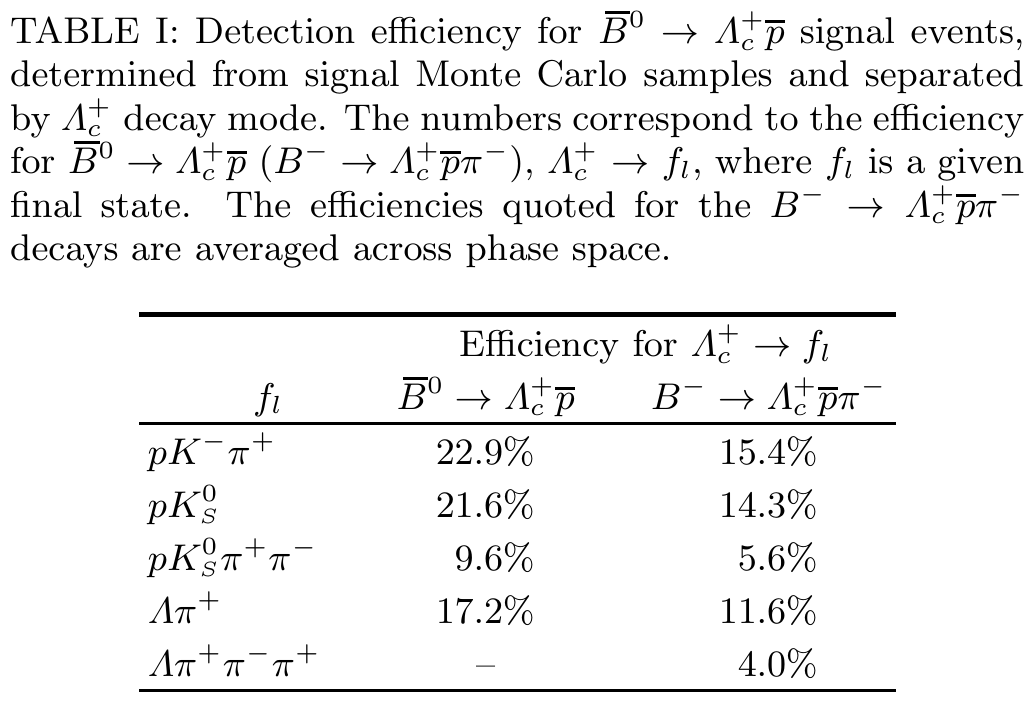
\includegraphics[width=.7\textwidth]{figures/002/table-efficiencies}

  %  + +0we reconstruct + Λc candidates in the pK −π , pKS 0, pK S π+ π− 
  %  , and Λπ decay modes, requiring the in- variant mass of each Λ+ 
  %  c candidate to be within 10 MeV/c 2 of the world average value [8].
  %
  %  For B − + → − Λc + + pπ − , we also reconstruct Λ+ c candidates in the 
  %  Λπ π π decay mode, and require all of the Λc + candidates to have an 
  %  invariant mass within 12 MeV/c2 of the world average value.
  %
  %  Ks -> 2pi
  %  Lambda -> p pi opposite
  %  both within 10 MeV
  %
  %  BKG: ee -> qq continuum + 
  % B 0 → Σc +p, Σc + → Λc+ π0

  % Efficiencies come from MC with kinematic reweighting.
  % Plus tracking inefficiencies from displaced vertices of intermediate 
  % particles.
  % 2D fit with mm and mr variables.
  % Bkg is threshold in mm with linear mr (same for data)
  % Threshold describes the beam energy.
  % Signal as Gaussian in mm and asymmetric Gauss in mr.

  % For the Lc ~p pi decay, the Dalitz plane is divided into bins based 
  % on kinematic parameters. Variations of efficiency across bins is of 
  % a factor of 2 and these 50\% drops are scarce.
  % The table shows average values for illustration.
\end{frame}%}}}

\begin{frame}[label=fit]%{{{
  \frametitle{Signal extraction}

  % 2D fit again in mm, mr. Sim fit of all the Lc decay modes. B0 and B- 
  % are fit separately.

  % Bkg is again threshold with linear in mr. Threshold parameter is 
  % common for all modes. The linear function is independent.

  % Signal is Gauss x Gauss for Lc ~p and
  % Gauss x double Gauss for Lc ~p pi.
  % Parameters common for modes.
  % Single Gauss for Lc ~p because of the small expected yield.

  % Results are found unbiased. Check based on MC signal events and 
  % toy-MC bkg events, which were both used to generate 100 
  % distributions.

  \parbox{.48\textwidth}{
    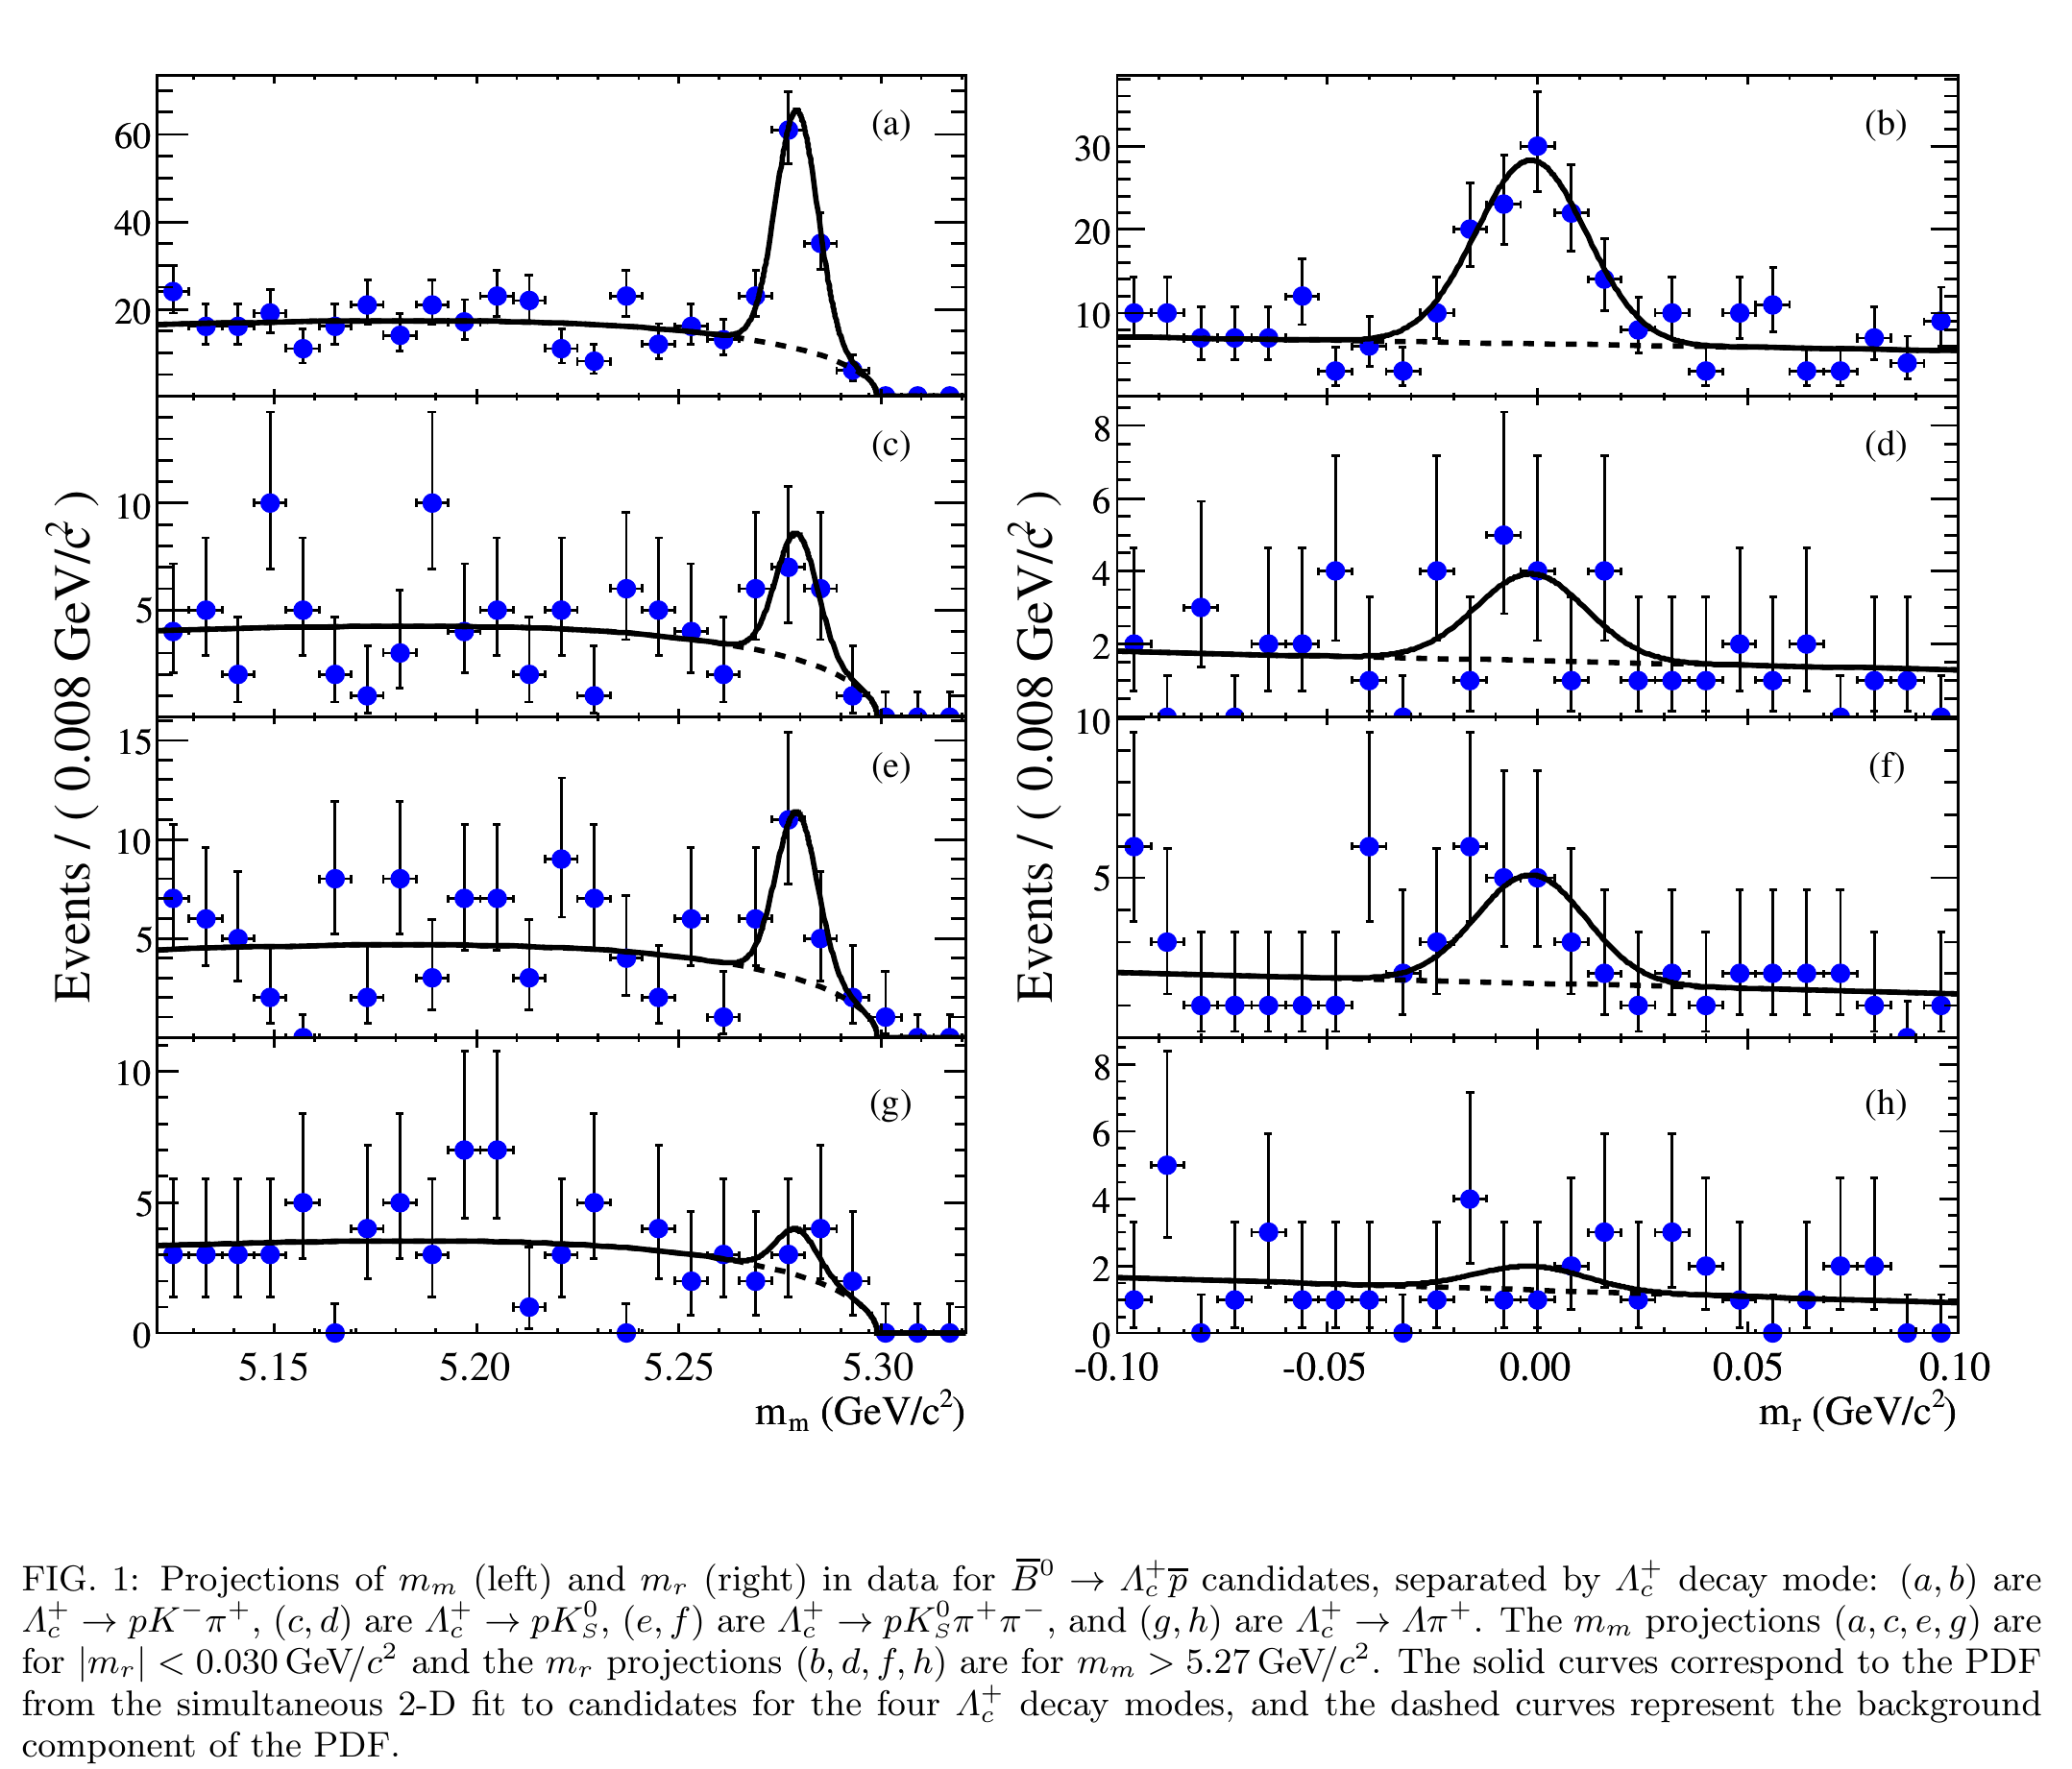
\includegraphics[width=\linewidth]{figures/002/fits-Lcp}
  } \parbox{.48\textwidth}{
    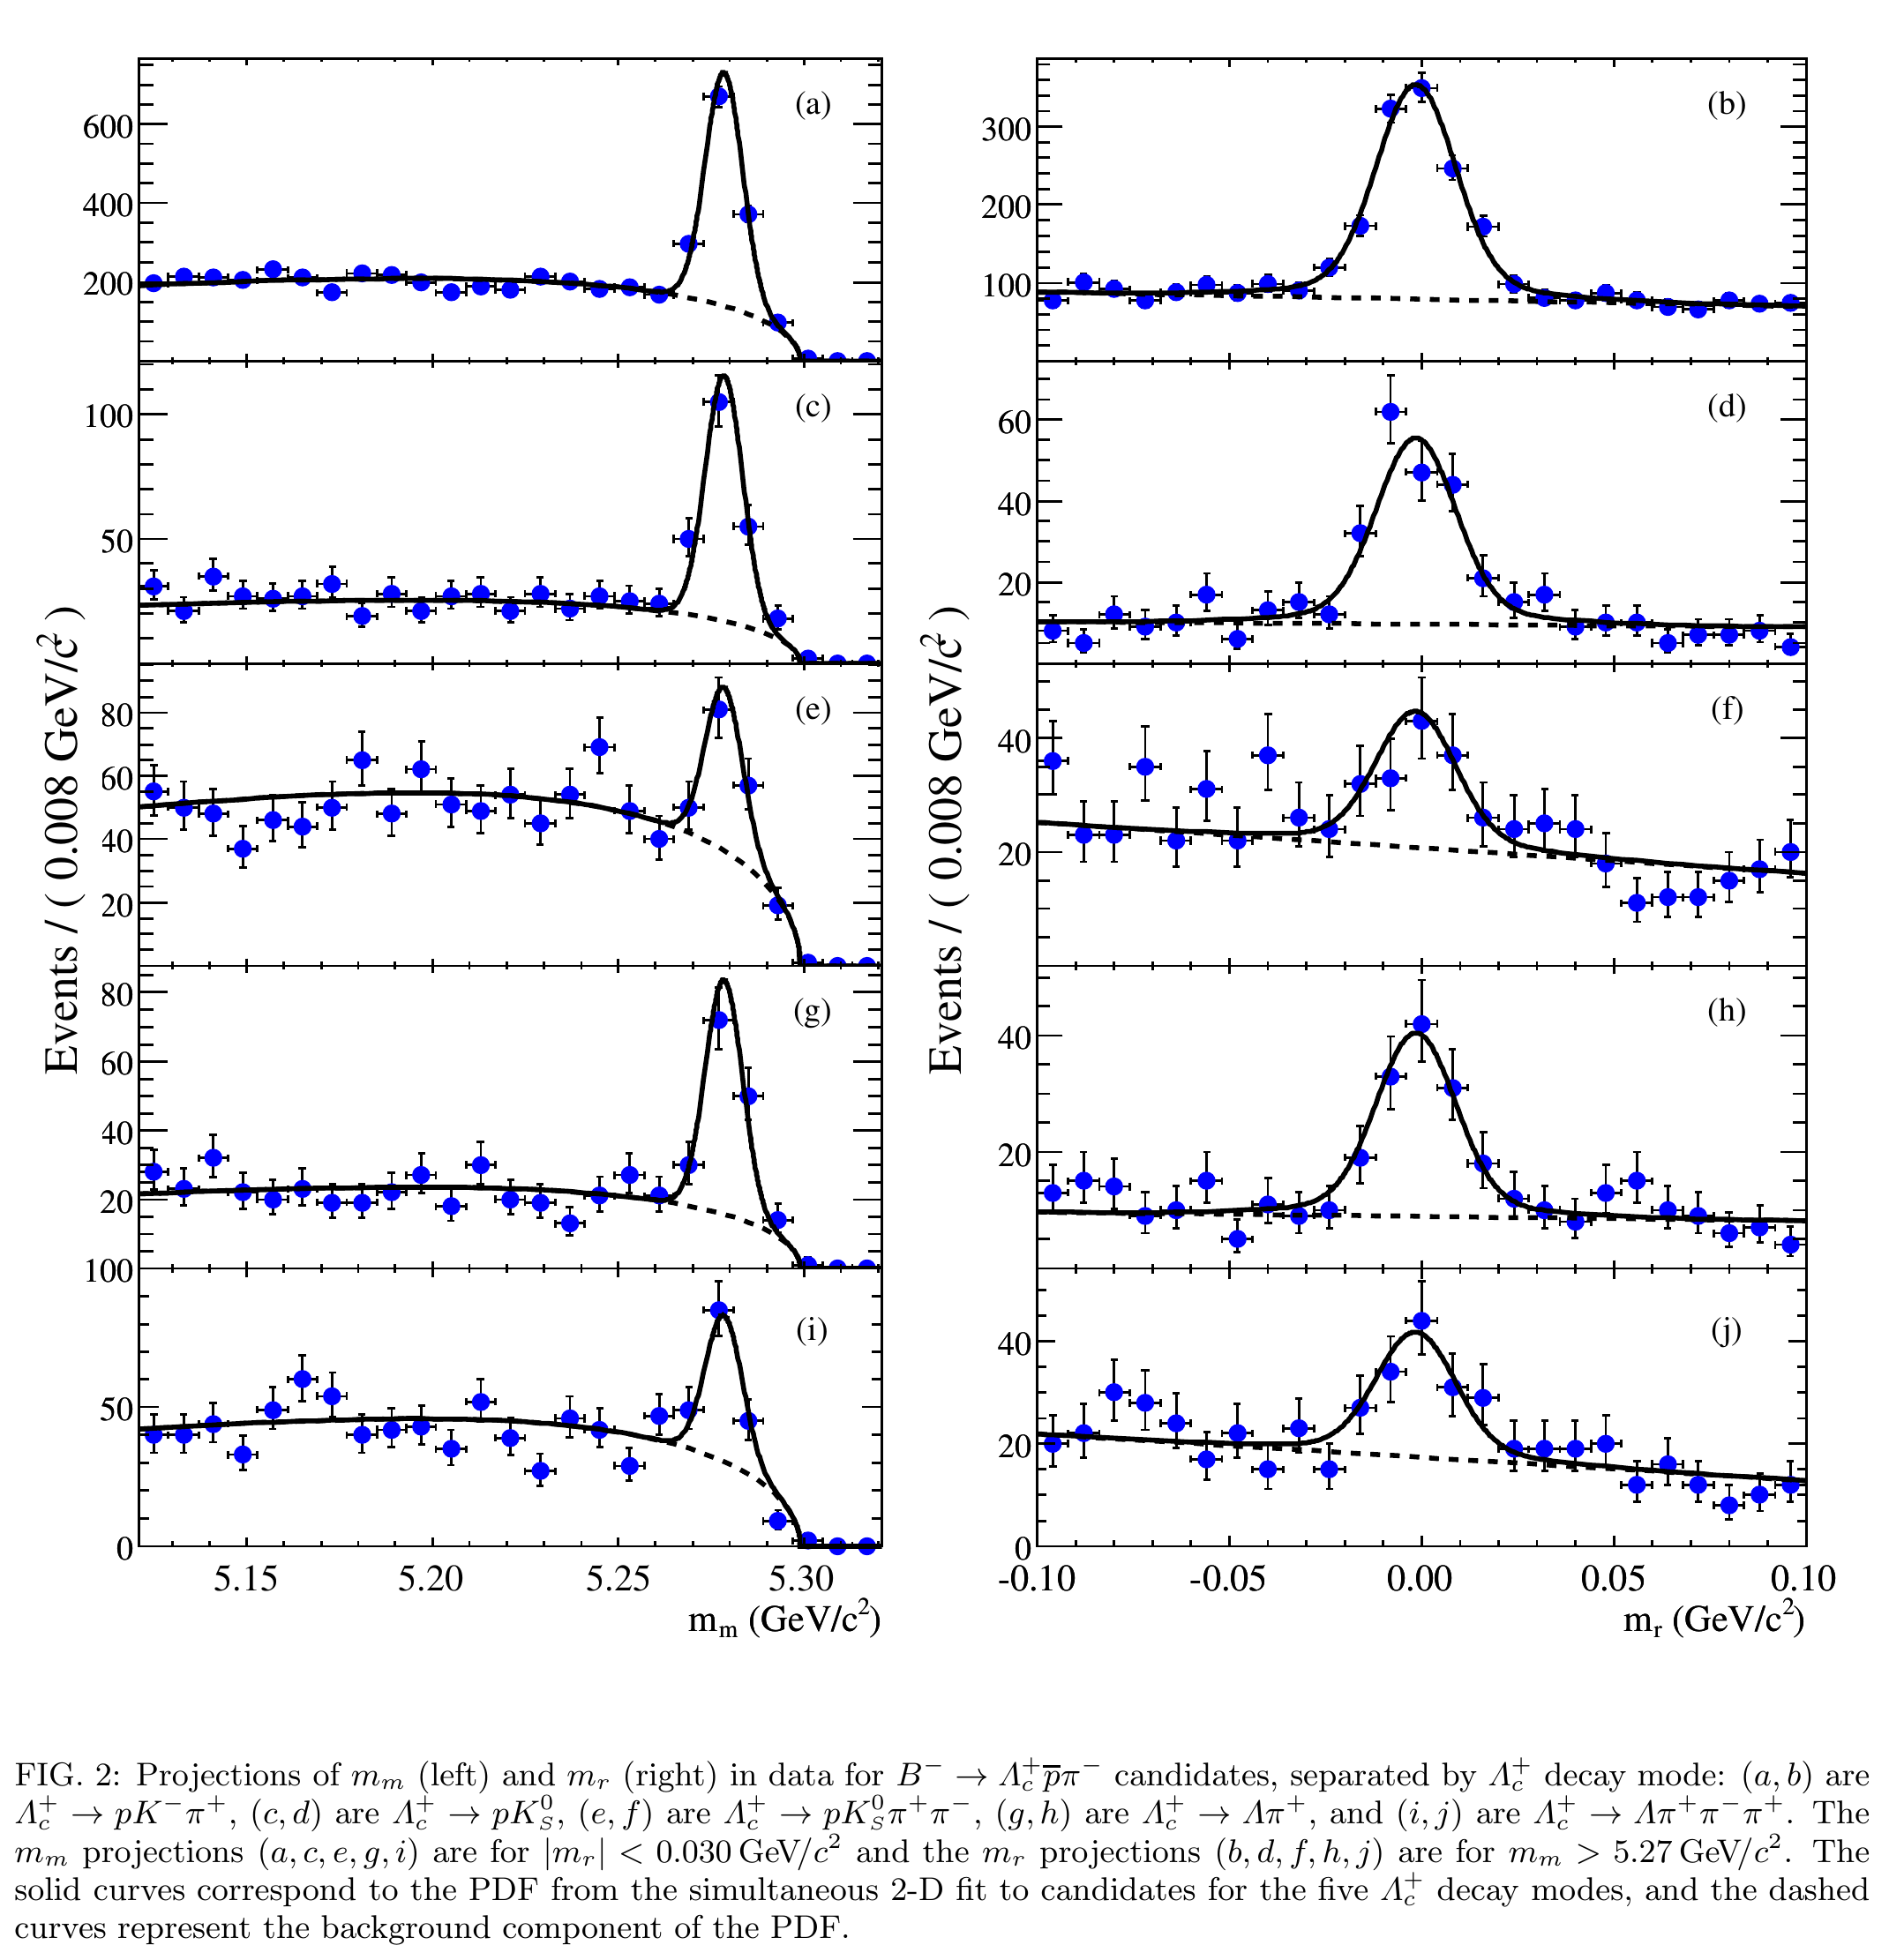
\includegraphics[width=\linewidth]{figures/002/fits-Lcppi}
  }
\end{frame}%}}}

\begin{frame}[label=fit-table]%{{{
  \frametitle{Fit results}
  \centering

  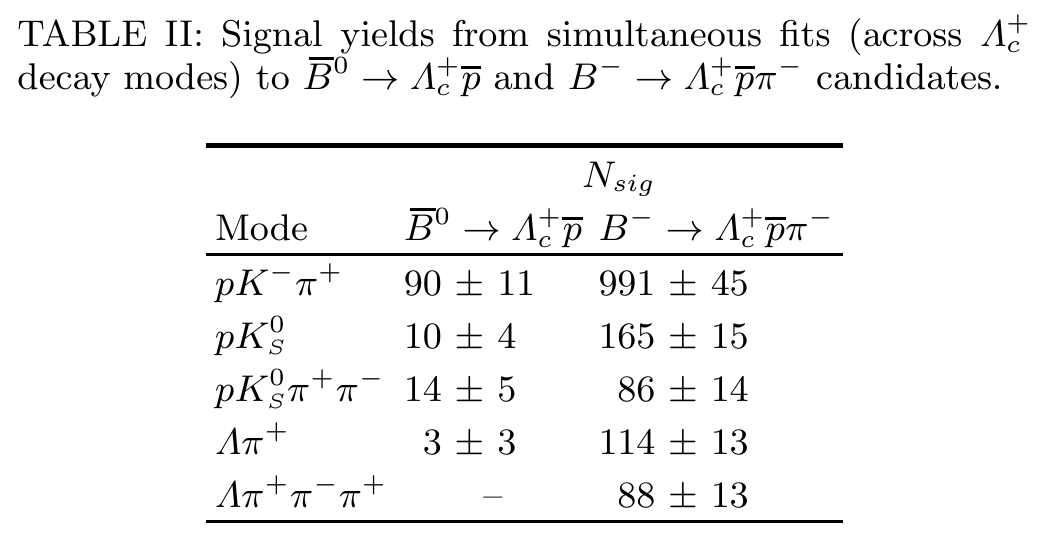
\includegraphics[width=.8\textwidth]{figures/002/table-yields}
\end{frame}%}}}

\begin{frame}[label=efficiency-correction]%{{{
  \frametitle{Efficiency correction}

  % Lc ~p pi fits are then used for sPlot. Each event is assigned an 
  % sWeight, and the sum of the weights for each event corrected for the 
  % efficiency for this event (based on its kinematic parameters) is 
  % used for BR calculations. 1\% correction for Sc events contribution.

  % This is performed for each Lc decay mode.
  % These results are considered correlated, and the BLUE method is used. 
  % BLUE gives an estimate as a linear combination, has no bias and 
  % minimum dispersion. This estimate requires the knowledge of covariance 
  % matrix. M is the sum of stat and syst. Stat from sim fit. Syst is only 
  % errors, not covariances.

  % Error matrices are added linearly, so one can quote them separately. 
  % And BaBar also quotes errors due to R Lc->pKpi. N_BB errors are 
  % added as they should.

  \vskip -2ex

  $$ \mathcal{B} \big( \overline{B}{}^0 \to \Lambda_c^+ \bar{p} \big)_l =
  \frac{N_{\mathrm{sig},\,l}}{N_{B\overline{B}} \cdot \varepsilon_l
  \cdot \mathcal{R}_l \cdot \mathcal{B}\big( \Lambda_c^+ \to p K^- \pi^+ \big)}$$

  $$ \mathcal{B} \big( {B}{}^- \to \Lambda_c^+ \bar{p} \pi^- \big)_l =
  \frac{0.99 \cdot \left(\sum\limits_i\dfrac{_sW_i}{\varepsilon_i}\right)}
  {N_{B\overline{B}} \cdot \mathcal{R}_l \cdot
  \mathcal{B}\big( \Lambda_c^+ \to p K^- \pi^+ \big)}$$

  \vskip 2ex

  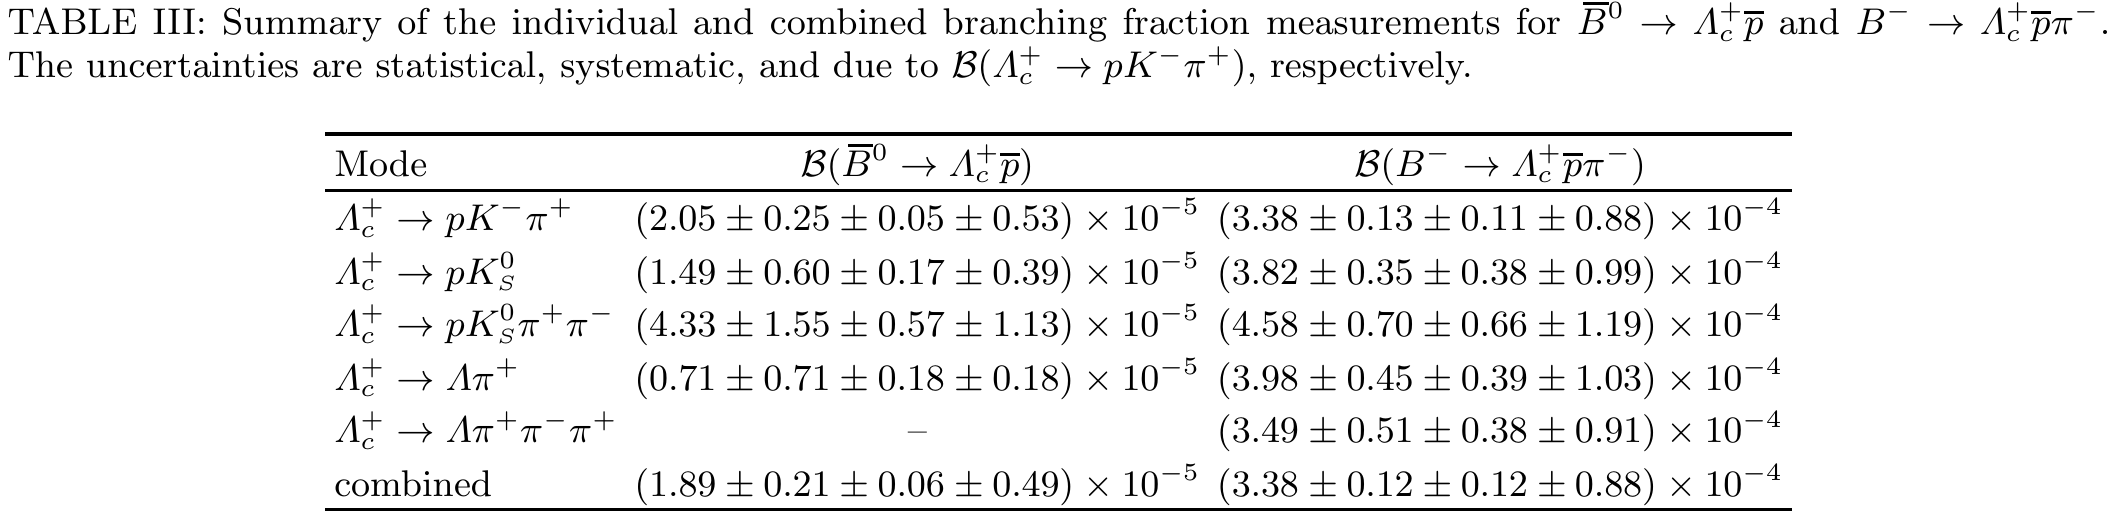
\includegraphics[width=\textwidth]{figures/002/table-corrected-yields}

  \pause
  \vskip -12ex
  \centering
  \large
  \colorbox{white}{\fbox{$
    \dfrac{\mathcal{B} \big( {B}{}^- \to \Lambda_c^+ \bar{p} \pi^- \big)}
    {\mathcal{B} \big( \overline{B}{}^0 \to \Lambda_c^+ \bar{p} \big)} =
    15.4 \pm 1.8 \pm 0.3
  $}}
  \vskip 12ex
\end{frame}%}}}

\begin{frame}[label=systematics]%{{{
  \frametitle{Systematic uncertainties}
  \centering
  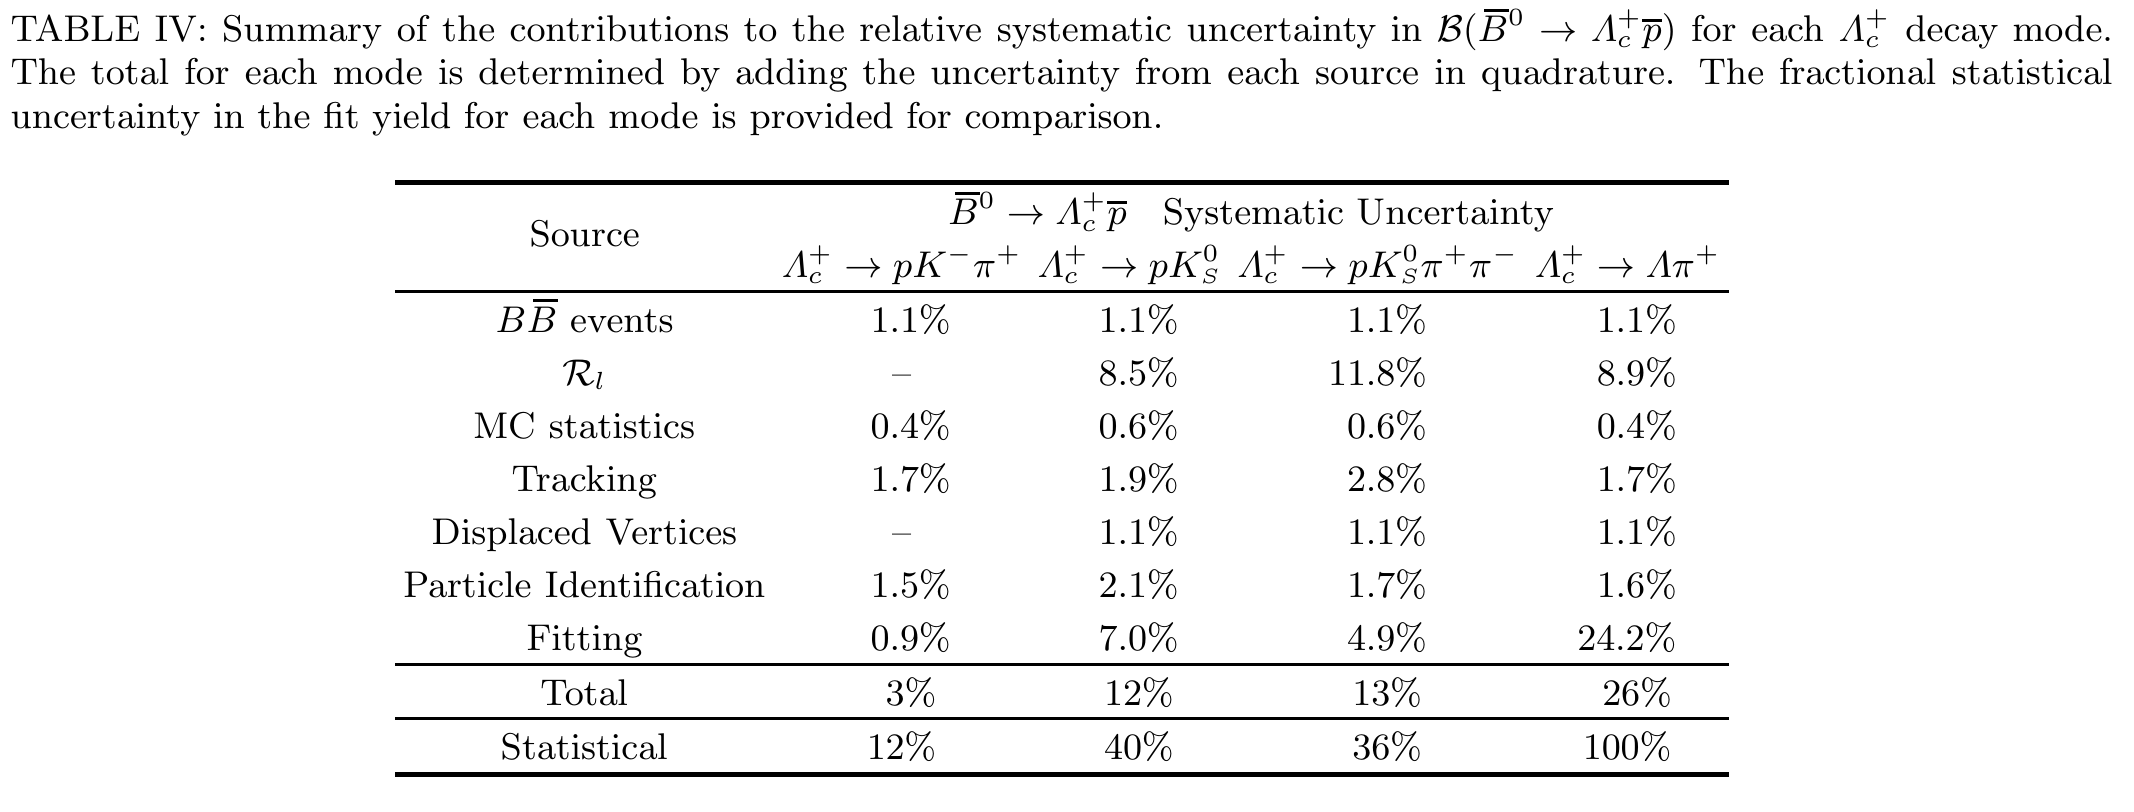
\includegraphics[width=.7\textwidth]{figures/002/table-syst-Lcp}
  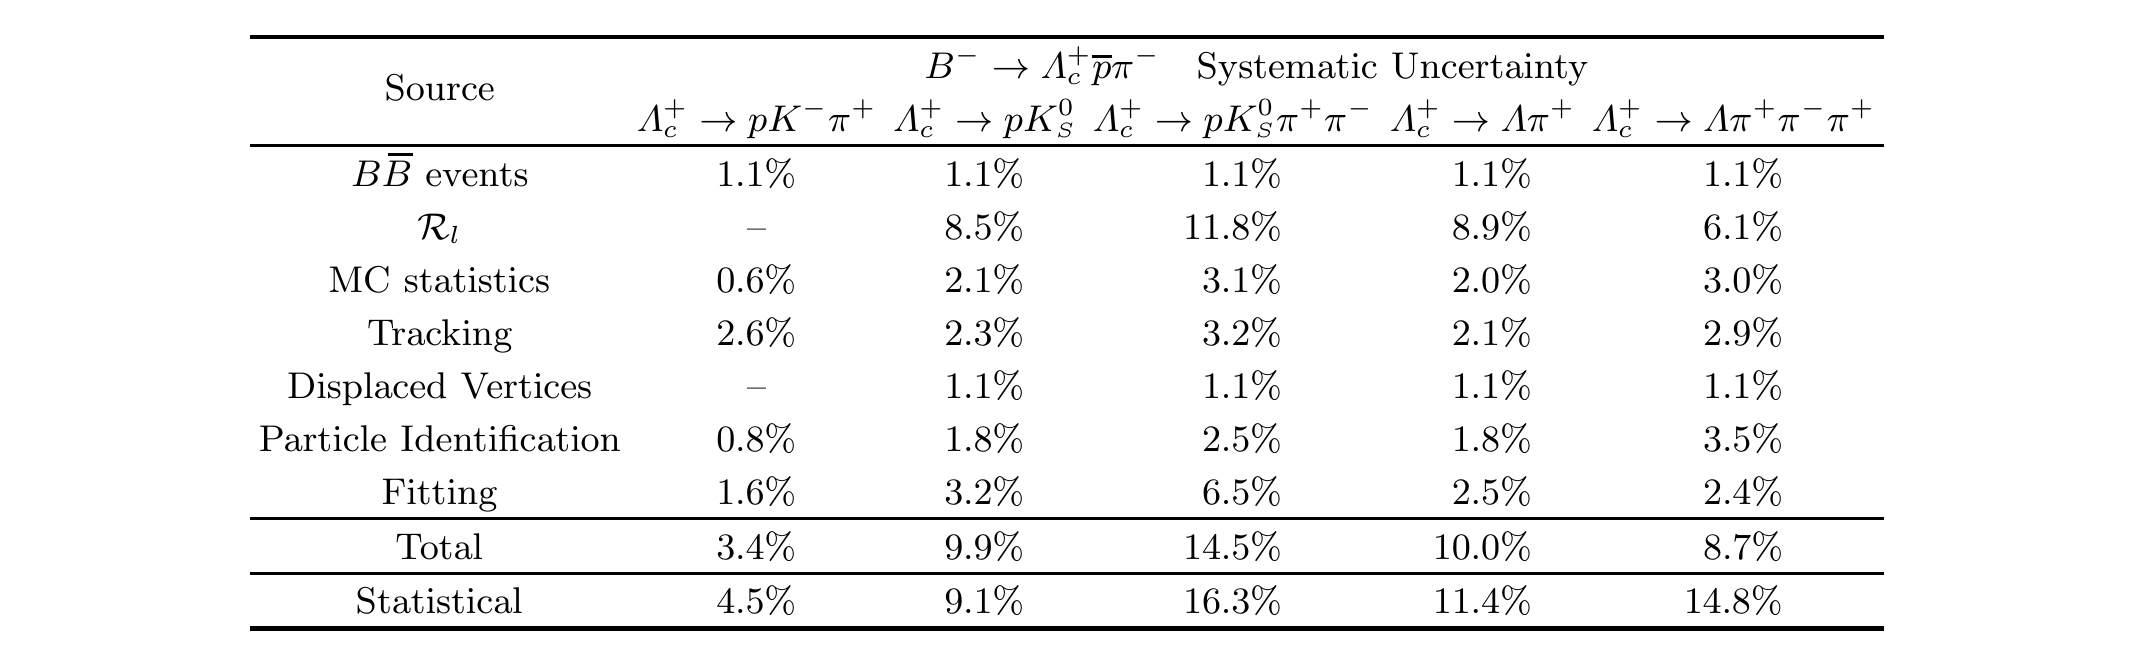
\includegraphics[width=.7\textwidth]{figures/002/table-syst-Lcppi-crop}

  % Largest error is due to Lc->pKpi decay.
  % Then Rl relative to it.
  % N_BB events is common.
  % Efficiencies and finite MC sample size. Per-bin for Lc~ppi.
  % Tracking -- how good the reconstruction is.
  % PID -- pid correction for MC and efficiencies.
  % Fit is due to bkg threshold common parameter (not common in check)
  % Fit also due to misreconstructed Sc~p, Sc->Lcpiz.
  % Fit also due to endpoint in m_m fit.
\end{frame}%}}}

\begin{frame}[label=resonances-sc2455]%{{{
  \frametitle{Resonant structure of $B^- \to \Lambda_c^+\bar{p}\pi^-$: 
              $\Sigma_c(2455)^0$}
  \centering

  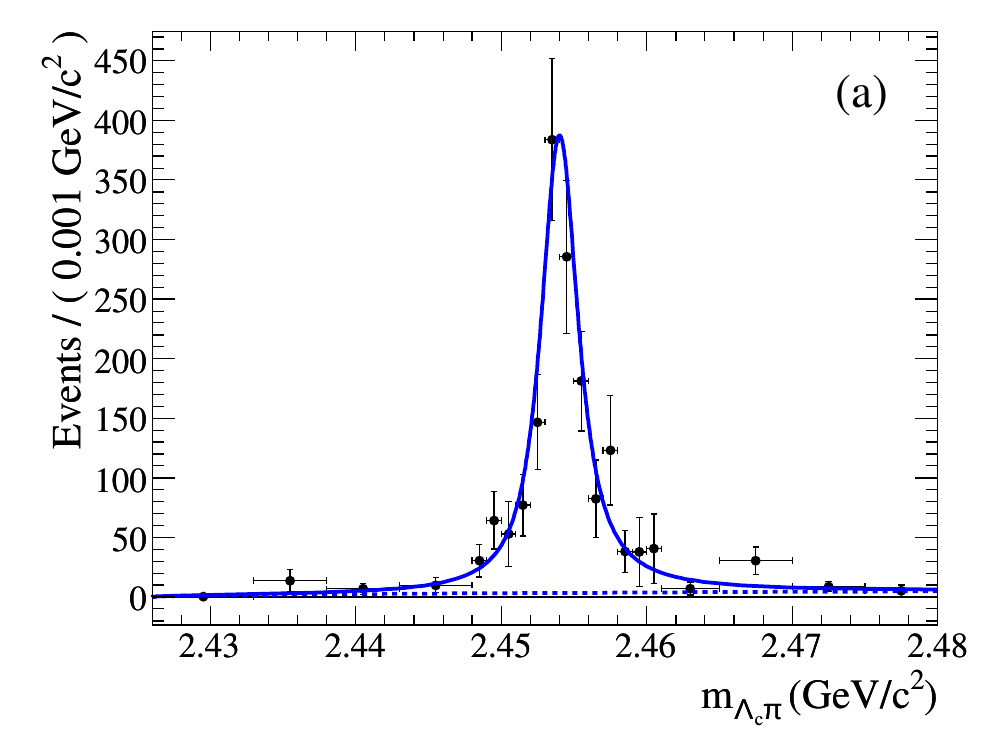
\includegraphics[width=.4\textwidth]{figures/002/fit-Sc2455}
  \hspace*{2ex}
  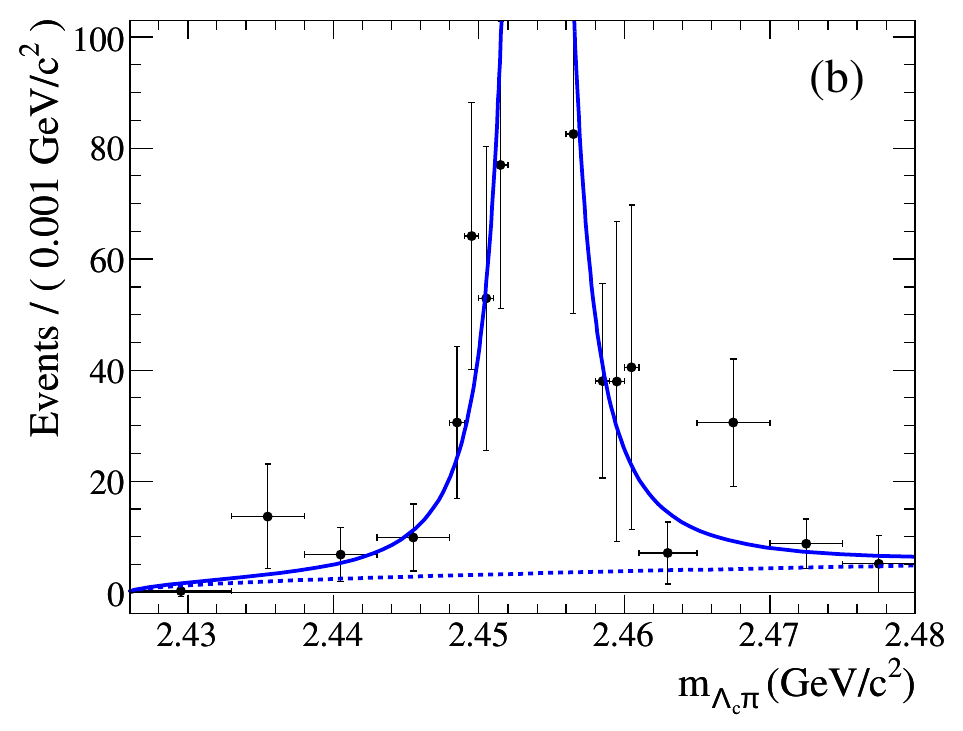
\includegraphics[width=.4\textwidth]{figures/002/fit-Sc2455-zoom}

  \small
  \begin{tabular}{lcc}
    \hline
    Fit parameter & Value & PDG value \\
    \hline
    $Y_\mathrm{sig}$ & $1522 \pm 149$ & -- \\
    $m_R$ (MeV$/c^2$) & $2454.0 \pm 0.2$ & $2453.8 \pm 0.2$ \\
    $\Gamma_R$ (MeV) & $2.6\pm0.5$ & $2.2\pm0.4$ \\
    \hline
  \end{tabular}

  % sPlot for mLcpi spectrum, chi2 binned fit. Variable bin width to 
  % ensure sufficient event counts and resolution around peaks.
  %
  % Only Sc2455 and Sc2800 are observed, no Sc2520.
  %
  % Sc2455 is S-wave BW conv with double Gauss resolution. Resolution is 
  % fixed to MC results. Bkg there is non-res decays: threshold 
  % function determined form MC NR events.
\end{frame}%}}}

\begin{frame}[label=resonances-sc2520]%{{{
  \frametitle{Resonant structure of $B^- \to \Lambda_c^+\bar{p}\pi^-$: $\Sigma_c(2520)^0$ -- no signal}
  \centering

  \hspace*{.15\textwidth}
  \parbox{.5\textwidth}{
    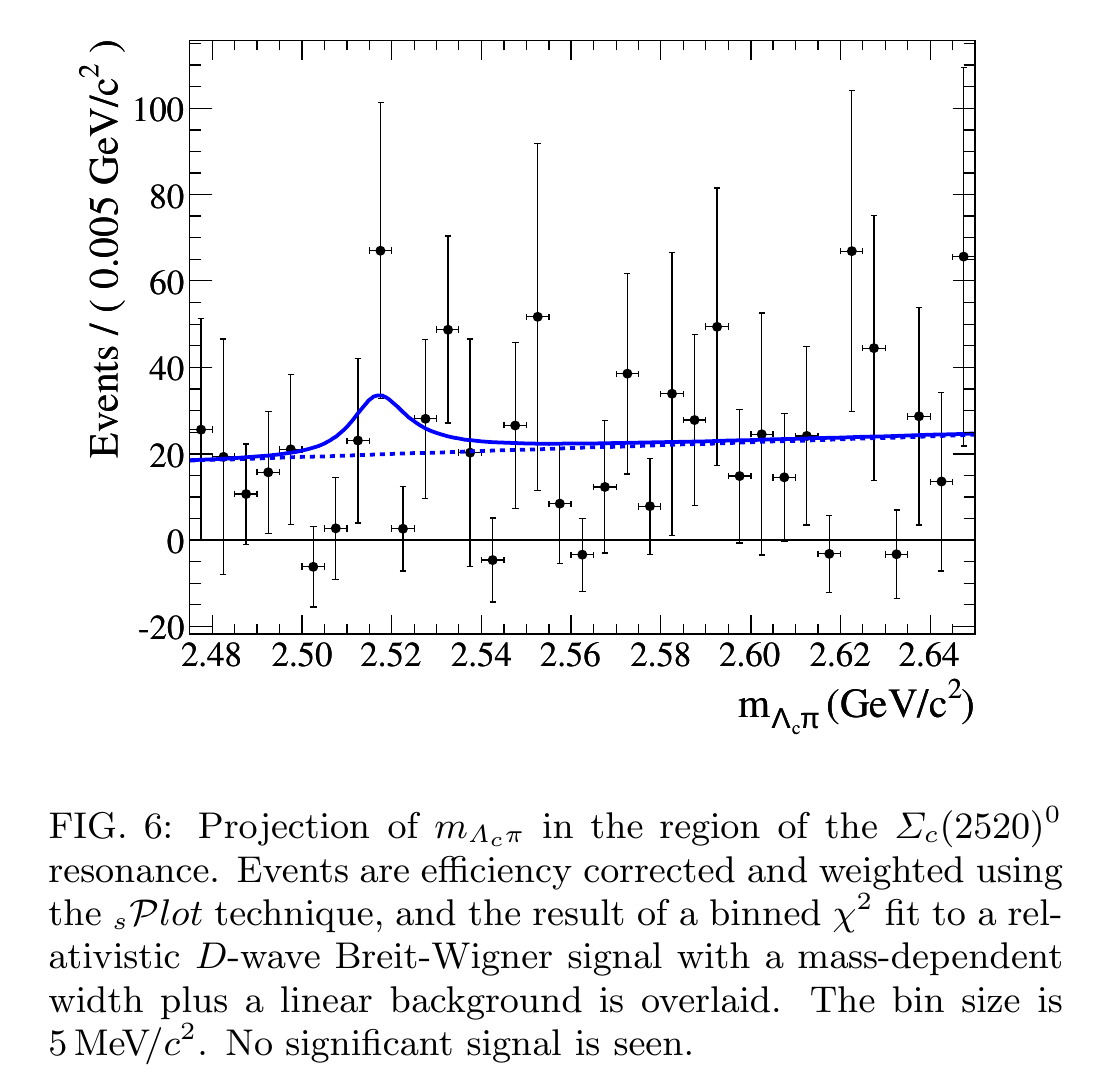
\includegraphics[width=\linewidth]{figures/002/fit-Sc2520}
  } \parbox{.2\textwidth}{
    % D-wave, linear NR bkg.
    \centering \small
    $Y_\mathrm{sig} = 27 \pm 69$
  }
\end{frame}%}}}

\begin{frame}[label=resonances-sc2800]%{{{
  \frametitle{Resonant structure of $B^- \to \Lambda_c^+\bar{p}\pi^-$: $\Sigma_c(2800)^0$}
  \centering

  \parbox{.45\textwidth}{
    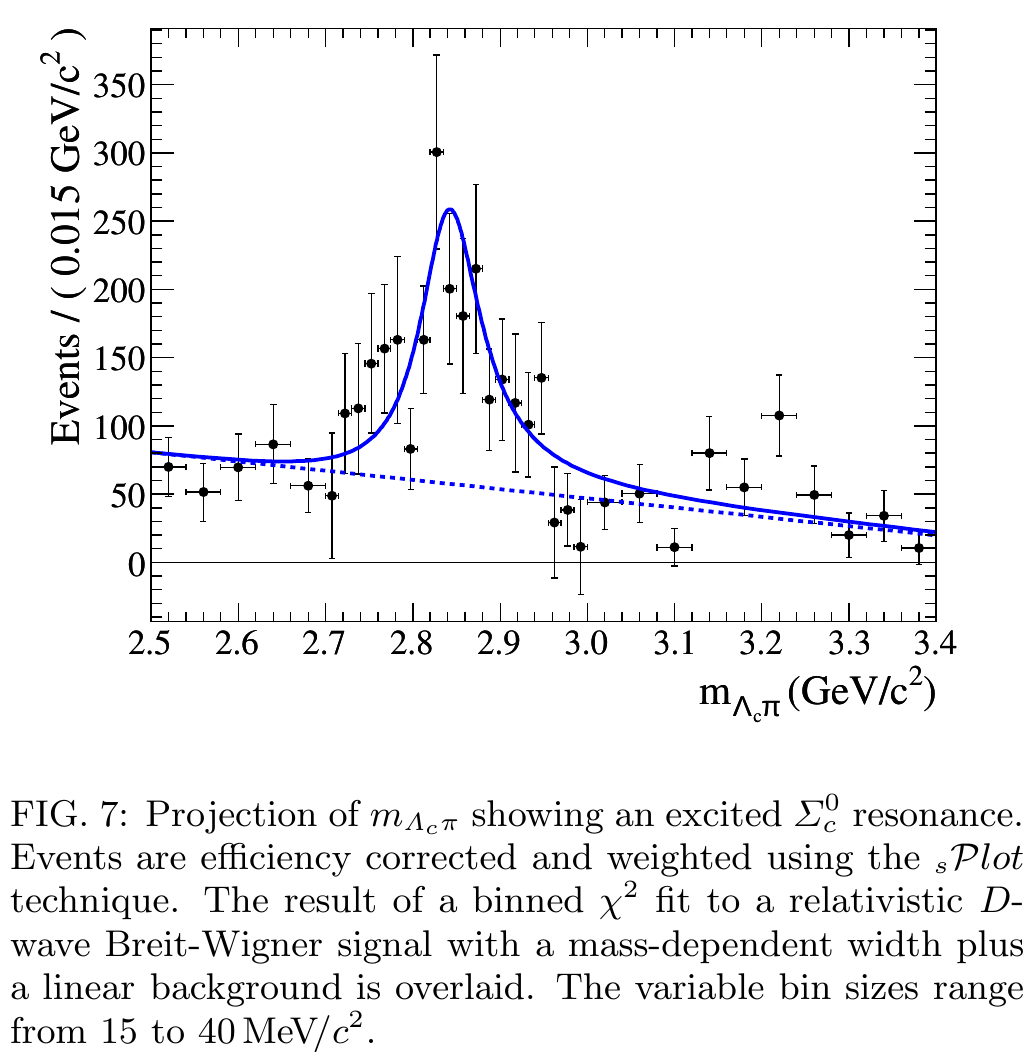
\includegraphics[width=\linewidth]{figures/002/fit-Sc2800}
  } \parbox{.45\textwidth}{
    % S, P, D waves checked. Mass-dependent width. No resolution because 
    % of the wide peak. D-wave baseline with S, P syst.
    % Linear NR bkg.
    \centering \small
    \begin{tabular}{lcc}
      \hline
      Fit parameter & Value & PDG value \\
      \hline
      $Y_\mathrm{sig}$ & $1449 \pm 284$ & -- \\
      $m_R$ (MeV$/c^2$) & $2846 \pm 8$ & $2802 ^{+4} _{-7}$ \\
      $\Gamma_R$ (MeV) & $86^{+33}_{-22}$ & $61^{+28}_{-18}$ \\
      \hline
    \end{tabular}
    \vskip 2ex \normalsize
    $5.8\sigma$ significance \\
    $5.2\sigma$ with systematics
  }
\end{frame}%}}}

\begin{frame}[label=res-syst]%{{{
  \frametitle{Systematic uncertainties of resonance parameters}
  \centering
  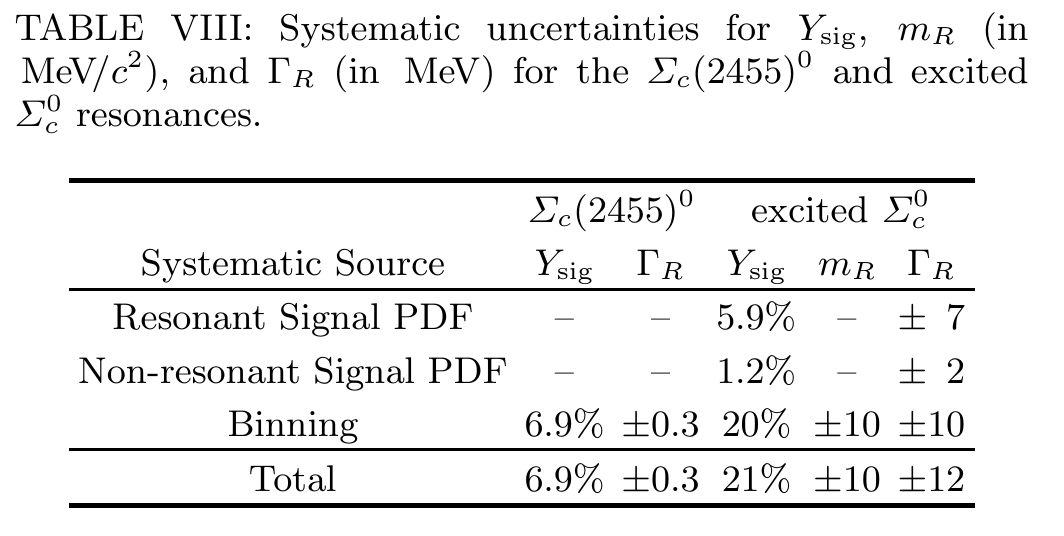
\includegraphics[width=.7\textwidth]{figures/002/table-syst-resonances}
  % Binning, resonant signal PDF, NR bkg PDF.
  % Binning decreased from 1 to .5 MeV for Sc2455
  % Binning varied from 10 to 20 MeV for Sc2800
  % PDF signal S, P waves.
  % PDF bkg threshold varied within MC fit error.
  % PDF bkg 2-order polynomial for Sc2800.
  %
  % Cross-checks:
  % - check for Delta resonance contrib. by limiting m(ppi) to higher 
  %   than its mass.
  % - check for Sc2800 presence in all Lc modes. Full data split into 
  %   mode Lc->pKpi and all others. The sum is ok, the relative numbers 
  %   are consistent with independence of Sc2800 of Lc modes.
\end{frame}%}}}

\begin{frame}[label=res-BRs]%{{{
  \frametitle{Resonant structure of $B^- \to \Lambda_c^+\bar{p}\pi^-$: Branching ratios}
  \Large

  $$ \frac{\mathcal{B}\big(B^- \to \Sigma_c(2455)^0 \bar{p} \big)}
  {\mathcal{B}\big(B^- \to \Lambda_c^+ \bar{p} \pi^- \big)}
  = \left(12.3 \pm 1.2 \pm 0.8 \right) \times 10^{-2}$$

  $$ \frac{\mathcal{B}\big(B^- \to \Sigma_c(2800)^0 \bar{p} \big)}
  {\mathcal{B}\big(B^- \to \Lambda_c^+ \bar{p} \pi^- \big)}
  = \left(11.7 \pm 2.3 \pm 2.4 \right) \times 10^{-2}$$

  $$ \frac{\mathcal{B}\big(B^- \to \Sigma_c(2520)^0 \bar{p} \big)}
  {\mathcal{B}\big(B^- \to \Lambda_c^+ \bar{p} \pi^- \big)}
  < 0.9 \times 10^{-2} \text{ (90\% C.L.)}$$
\end{frame}%}}}

\begin{frame}[label=sc2455-spin]%{{{
  \frametitle{$\Sigma_c(2455)$ spin measurement}
  % Degraded in exp due to nonuniform efficiencies, bkg events, theta_h 
  % resolution.
  %
  % Bkg is measured by abandoning sPlot, using mass cut, and looking at 
  % the Sc2455 signal and sidebands. The number of bkg events is ~ 5%
  %
  % Helicity angle resolution is measured based on MC signal. Maximum 
  % RMS of cos theta is found to be small compared to the functions.
  %
  % lnL is calculated as sum of efficiencies times lnPDF.
  % The ideal distributions are each used to generate 500 samples. For 
  % each sample, log L is evaluated for both JP hypotheses, and the 
  % difference is recorded.

  $B^- \to \Sigma_c(2455)^0 \big(\to\Lambda_c^+ \pi^-\big) \bar{p}$: \hfill
  $\theta_h$ is the angle between $\Lambda_c^+$ and $\bar{p}$ in $\Sigma_c(2455)^0$ rest frame.
  \hfill\null

  \vskip 2ex

  Ideal distributions for $J^P = 1/2$ and $3/2$:
  \[ \begin{aligned}
    J^P(\Sigma_c(2455)^0) = \frac{1}{2}: \quad \frac{\mathrm{d}N}{\mathrm{d}\cos\theta_h}
    \propto 1
    \qquad \qquad \qquad
    J^P(\Sigma_c(2455)^0) = \frac{3}{2}: \quad \frac{\mathrm{d}N}{\mathrm{d}\cos\theta_h}
    \propto 1 + 3 \cos^2 \theta_h
  \end{aligned} \]

  \vskip 2ex

  \parbox{.48\textwidth}{\centering
    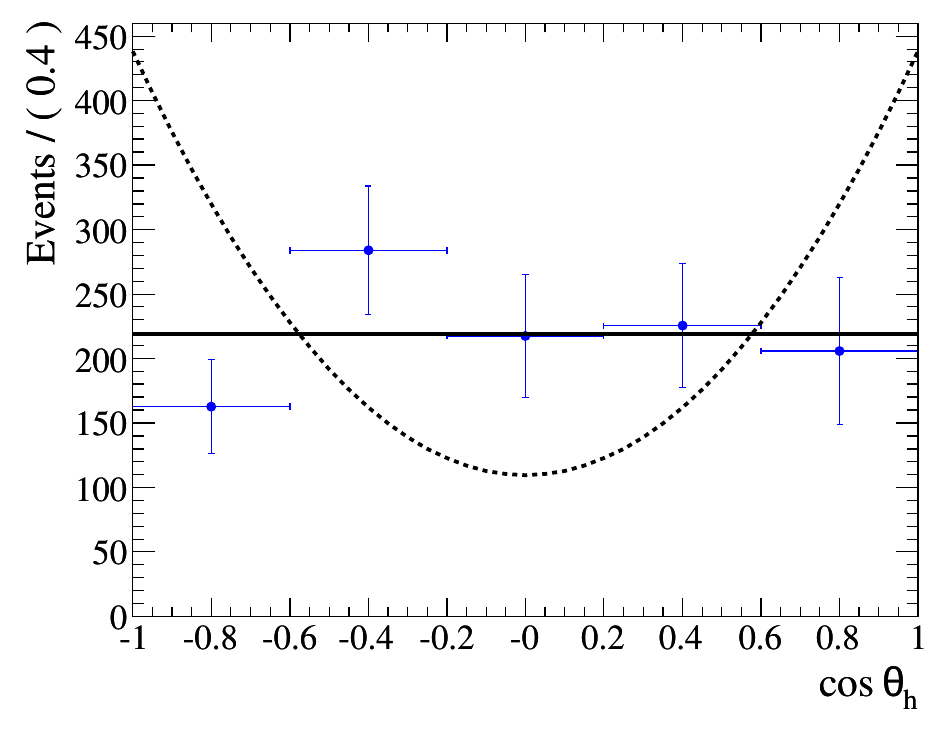
\includegraphics[width=.3\textwidth]{figures/002/angle-distribution}
  } \parbox{.48\textwidth}{\centering
    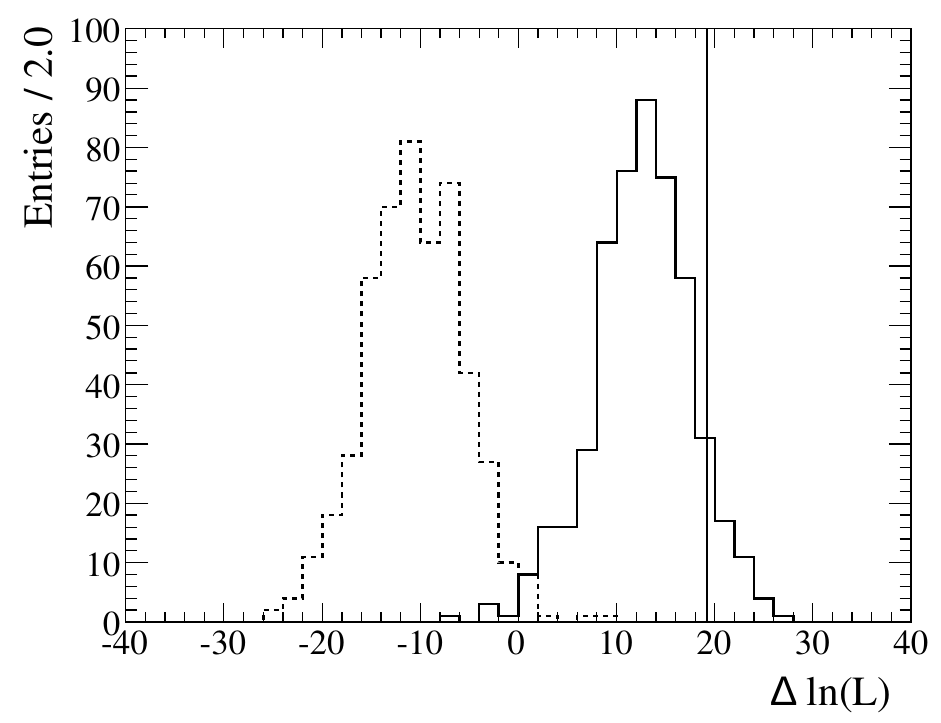
\includegraphics[width=.3\textwidth]{figures/002/spin-deltaL}
  }
\end{frame}%}}}

\begin{frame}[label=conclusion]%{{{
  \frametitle{Conclusions}
  \Large

  \begin{itemize}
    \item $\overline{B}{}^0 \to \Lambda_c^+ \bar{p}$ and
      $B^- \to \Lambda_c^+ \bar{p} \pi^-$ BR measurements,
    \item Measurement of their ratio,
    \item BRs of $B^-$ decays via $\Sigma_c(2455)^0$, $\Sigma_c(2800)^0$,
      % Supports theory that closer p~p decays are favored.
    \item $\Sigma_c(2455)^0$ spin consistent with $J^P = \frac{1}{2}^+$,
    \item $\Sigma_c(2455)^0$ and $\Sigma_c(2800)^0$ masses and widths measured.
  \end{itemize}
\end{frame}%}}}

\end{document}


Vocabulary:

enhancement 
laboratory for a range of particle physics investigations
pentaquark
glueball
angular distributions
flavor-changing neutral currents 
pole models
diquark models
decays weakly
baryon production
baryon production mechanisms
e+ e− asymmetric-energy B Factory
axial magnetic field
Charged particle identification
Cherenkov radiation detection
ring-imaging detector
Exclusive B-meson decays
generic hadronization processes.
Fisher
discriminant
B candidate thrust axis
uncorrelated alternative
energy-substituted mass
continuum e+ − e− → qq events
probability distribution function
extended unbinned maximum
likelihood fit
transpose
isospin partners
coarse regions
